% \RequirePackage{filecontents}
% \begin{filecontents}{\jobname.bib}
% @article{qian1999momentum,
% title={On the momentum term in gradient descent learning algorithms},
% author={Qian, Ning},
% journal={Neural networks},
% volume={12},
% number={1},
% pages={145-151},
% year={1999},
% publisher={Elsevier}
% }
% \end{filecontents}


\documentclass{beamer}

\mode<presentation> {
\usetheme{Boadilla}
\usecolortheme{default}
}
%\usepackage{natbib}
\usepackage{amsmath}
\usepackage{amssymb}
\usepackage{amsthm}
\usepackage[USenglish,british,american,australian,english]{babel}
%\usepackage{bibentry}
%\usepackage[backend=biber]{biblatex}
\begin{filecontents}{\jobname.bib}
@article{qian1999momentum,
  title={On the momentum term in gradient descent learning algorithms},
  author={Qian, Ning},
  journal={Neural networks},
  volume={12},
  number={1},
  pages={145--151},
  year={1999},
  publisher={Elsevier}
}
\end{filecontents}
\usepackage[style=numeric,backend=biber,autocite=plain,sorting=none]{biblatex}
\addbibresource{\jobname.bib}
  
\usepackage{graphicx} % Allows including images
\usepackage{booktabs} % Allows the use of \toprule, 
\usepackage{listings}
\usepackage{minted}
\usepackage{tikz}
%\usepackage{etoolbox} % for \ifthen
\usepackage{listofitems} % for \readlist to create arrays
\usetikzlibrary{arrows.meta} % for arrow size
\usepackage[outline]{contour} % glow around text
\contourlength{1.4pt}

\tikzset{>=latex} % for LaTeX arrow head
\usepackage{xcolor}
\colorlet{myred}{red!80!black}
\colorlet{myblue}{blue!80!black}
\colorlet{mygreen}{green!60!black}
\colorlet{myorange}{orange!70!red!60!black}
\colorlet{mydarkred}{red!30!black}
\colorlet{mydarkblue}{blue!40!black}
\colorlet{mydarkgreen}{green!30!black}
\tikzstyle{node}=[thick,circle,draw=myblue,minimum size=22,inner sep=0.5,outer sep=0.6]
\tikzstyle{node in}=[node,green!20!black,draw=mygreen!30!black,fill=mygreen!25]
\tikzstyle{node hidden}=[node,blue!20!black,draw=myblue!30!black,fill=myblue!20]
\tikzstyle{node convol}=[node,orange!20!black,draw=myorange!30!black,fill=myorange!20]
\tikzstyle{node out}=[node,red!20!black,draw=myred!30!black,fill=myred!20]
\tikzstyle{connect}=[thick,mydarkblue] %,line cap=round
\tikzstyle{connect arrow}=[-{Latex[length=4,width=3.5]},thick,mydarkblue,shorten <=0.5,shorten >=1]
\tikzset{ % node styles, numbered for easy mapping with \nstyle
  node 1/.style={node in},
  node 2/.style={node hidden},
  node 3/.style={node out},
}
\def\nstyle{int(\lay<\Nnodlen?min(2,\lay):3)} % map layer number onto 1, 2, or 3
\DeclareMathOperator*{\argmax}{arg\,max}
\DeclareMathOperator*{\argmin}{arg\,min}

%Includes "References" in the table of contents

\title[CodeSeoul] % (optional, only for long titles)
	{Optimization algorithms in deep learning}

\author[AI *** Research Paper Review] % (optional, for multiple authors)
	{Sanzhar Askaruly}

\institute[] % (optional)
	{ Ulsan National Institute of Science and Technology\newline
	  Ph.D. Candidate in Biomedical Engineering}

\date{\today} 

% some change
\begin{document}
    %\maketitle
    \begin{frame}
    \titlepage % Print the title page as the first slide
    \end{frame}

    % \begin{frame}
    % \frametitle{Overview} % Table of contents slide, comment this block out to remove it
    % \tableofcontents 
    % \end{frame}

    \begin{frame}{Optimization}
      \begin{center}
        \begin{huge}
          In \textit{context} of deep learning, \\
          goal is to \textbf{minimize loss function}
          \vspace{0.2cm}
          \begin{equation}
            \mathit{w}^* = \argmin_{w}L(w)
          \end{equation}
        \end{huge}
      \end{center}
    \end{frame}

    \begin{frame}{What is gradient descent optimization?}
      \begin{center}
          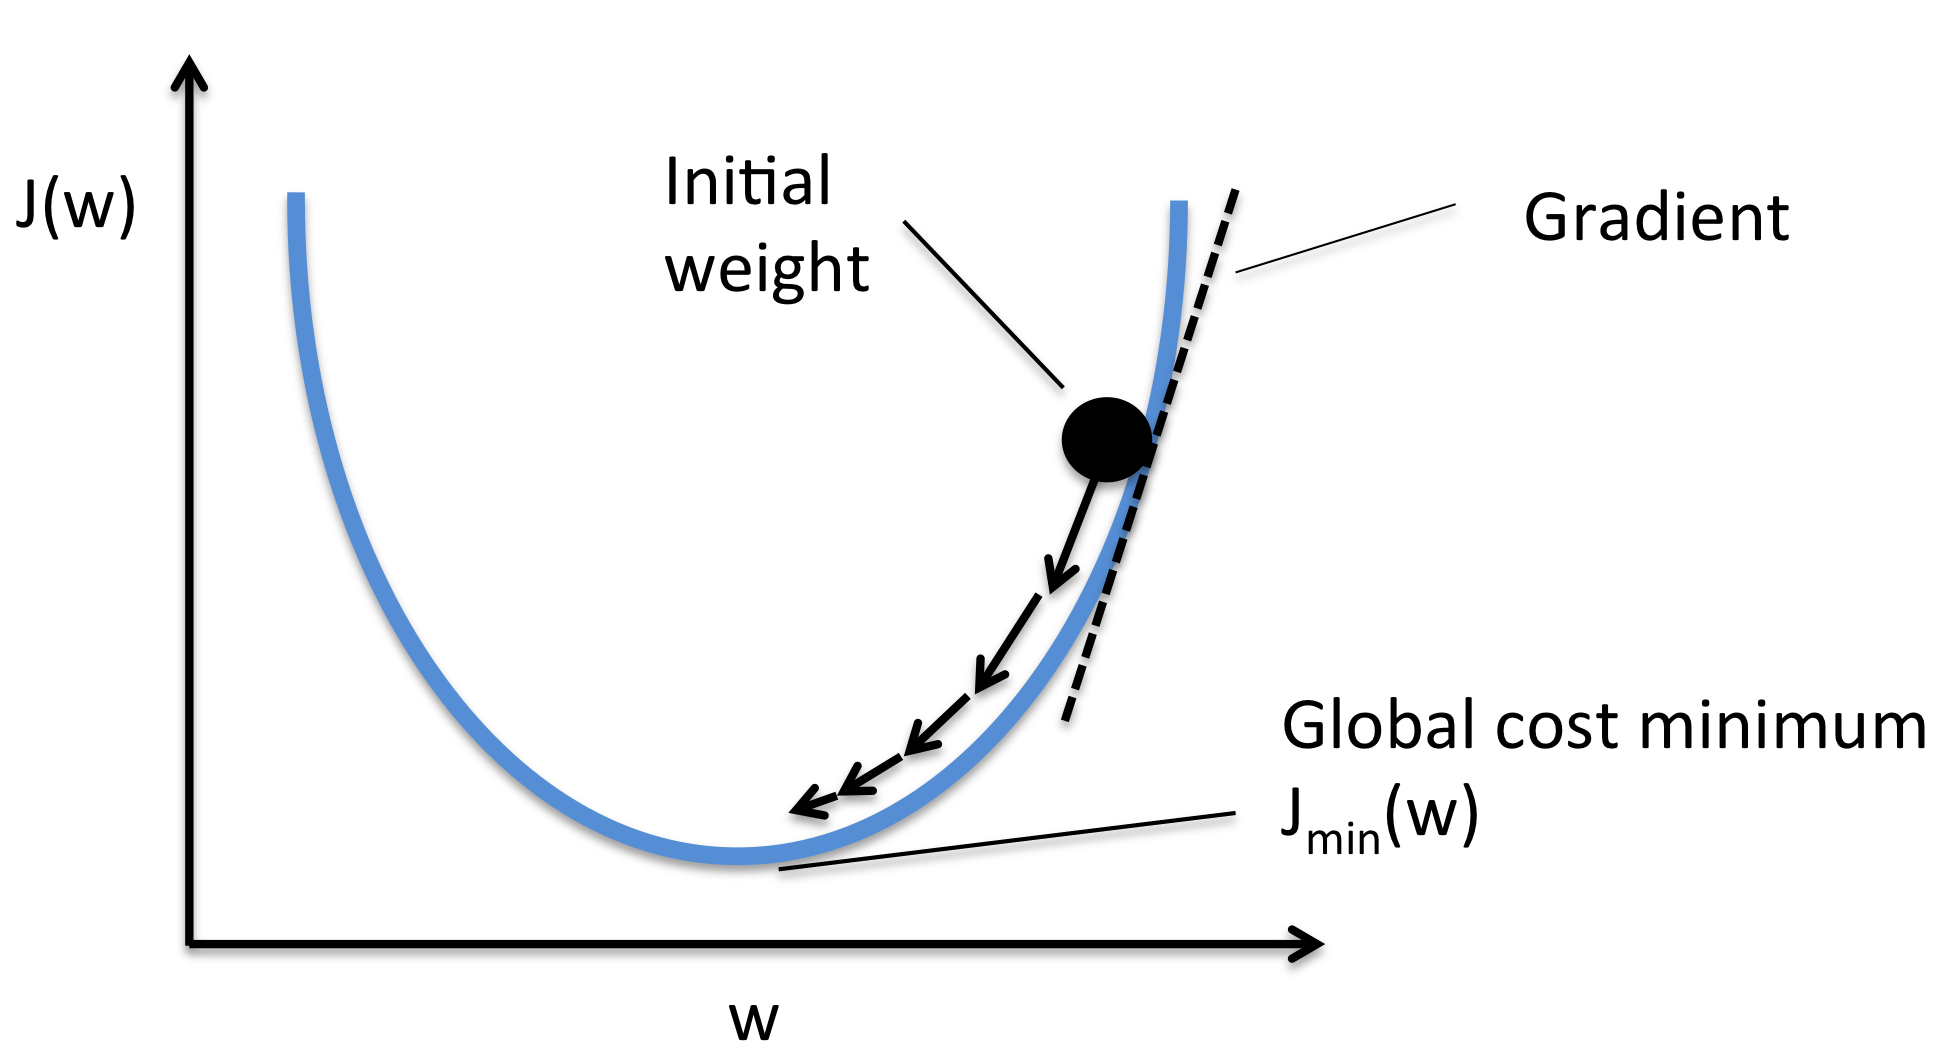
\includegraphics[width=0.8\textwidth]{/home/suzy/gitrepos/tuttelikz/221105/images/what_is_gd.png}
      \end{center}
    \end{frame}

    \begin{frame}
      \frametitle{Stochastic Gradient Descent (SGD)} % Table of contents slide, comment this block out to remove it
      \begin{block}{Algorithm}
        Update step:
        \begin{equation}
          \theta_{t+1} = \theta_{t} - \eta \cdot \nabla_{\theta}J(\theta_t)
        \end{equation}
        \vskip 0.3cm
        where, \\
        \begin{tabular}{l l}
          $\theta_{t}$: & current model parameters \\
          $\nabla_{\theta}J(\theta_t)$: & gradient of these model parameters \\
          $\eta$: & learning rate (fixed)
        \end{tabular}
        
      \end{block}
    \end{frame}


    \begin{frame}[fragile]
      \frametitle{Stochastic Gradient Descent (SGD)}
      \vspace{0.2cm}
      How we usually call in \verb|PyTorch|:
      \rule{\textwidth}{1pt}
      \scriptsize
      \begin{minted}{python}
        optimizer = optim.SGD(model.parameters(), lr=0.01)
      \end{minted}
      \rule{\textwidth}{1pt}
      
      \normalsize
      \vspace{0.2cm}
      How we can create our "native" class:
      \rule{\textwidth}{1pt}
      \scriptsize
      \begin{minted}{python}
        from torch.optim.optimizer import Optimizer
        
        class CustomSGD(Optimizer):
          def __init__(self, model_params, lr=1e-3):
              self.model_params = list(model_params)
              self.lr = lr

          def zero_grad(self):
              for param in self.model_params:
                  param.grad = None

          @torch.no_grad()
          def step(self):
              for param in self.model_params:
                  param.sub_(self.lr * param.grad)
      \end{minted}
      \rule{\textwidth}{1pt}
    \end{frame}

    \begin{frame}
      \frametitle{SGD with Momentum} % Table of contents slide, comment this block out to remove it
      
      \begin{columns}
          \begin{column}{0.5\textwidth}
            General idea:
            \begin{itemize}
              \item Overcome small gradients \\ near flat areas
              \item Build up from previous "velocity"
              \item Faster learning
            \end{itemize}
          \end{column}
          \begin{column}{0.5\textwidth}  %%<--- here
              \begin{center}
                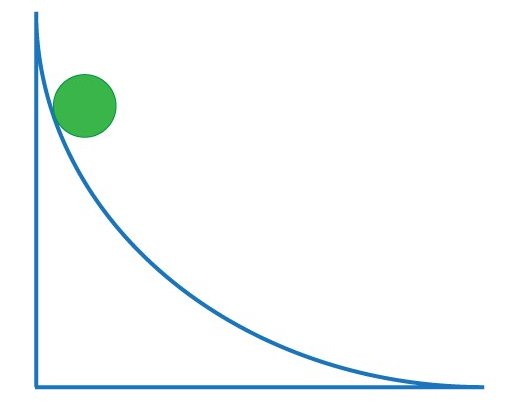
\includegraphics[width=0.8\textwidth]{/home/suzy/gitrepos/tuttelikz/221105/images/ball_momentum.jpeg}
              \end{center}
          \end{column}
      \end{columns}
    \end{frame}

    \begin{frame}
      \frametitle{SGD with Momentum}
      \begin{block}{Algorithm}

        Update step ~\cite{qian1999momentum}:
        \begin{equation}    % <--- deleted empty lines
          v_{t,i} = \gamma \cdot v_{t-1,i} + \nabla_{\theta}J(\theta_{t,i})
        \end{equation}
        \begin{equation}    % <--- deleted empty lines
          \theta_{t+1} = \theta_{t} - \eta \cdot v_{t,i}
        \end{equation}

        \vskip 0.3cm
        where, \\
        \begin{tabular}{l l}
          $\gamma$: & friction (or momentum, fixed) \\
          $v_{t}$: & velocity \\
          $\nabla_{\theta}J(\theta_t)$: & gradient of these model parameters \\
          $\eta$: & learning rate (fixed)
        \end{tabular}
      \end{block}
    \end{frame}



    \begin{frame}[fragile]
      \frametitle{SGD with Momentum}
      \vspace{0.2cm}
      \rule{\textwidth}{1pt}
      \scriptsize
      \begin{minted}{python}
        from torch.optim.optimizer import Optimizer

        class CustomSGDMomentum(Optimizer):
          def __init__(self, model_params, lr=1e-3, momentum=0.9):
              self.model_params = list(model_params)
              self.lr = lr
              self.momentum = momentum
              self.v = [torch.zeros_like(p) for p in self.model_params]

          def zero_grad(self):
              for param in self.model_params:
                  param.grad = None

          @torch.no_grad()
          def step(self):
              for param, v in zip(self.model_params, self.v):
                  v.mul_(self.momentum).add_(param.grad)
                  param.sub_(self.lr * v)
      \end{minted}
      \rule{\textwidth}{1pt}
    \end{frame}




    \begin{frame}
      \begin{center}
      \frametitle{SGD with Momentum~\cite{qian1999momentum}}
      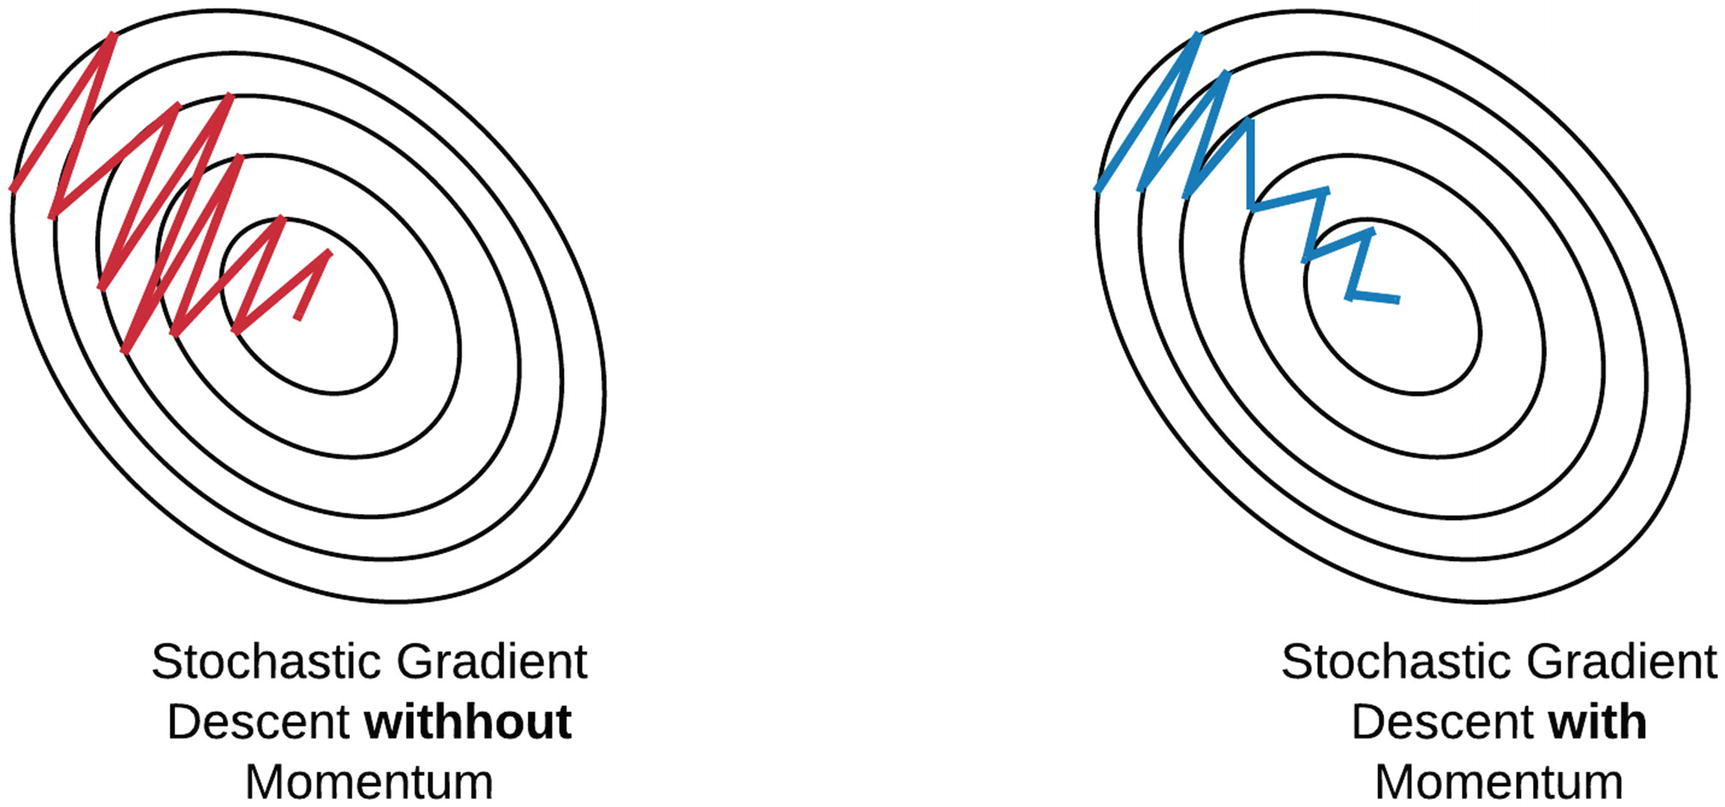
\includegraphics[width=0.8\textwidth]{/home/suzy/gitrepos/tuttelikz/221105/images/momentum.jpeg}
      \end{center}
    \end{frame}



    \begin{frame}{Experiment}
    \begin{flushleft}
      A vanilla MLP (Multilayer Perceptron)
    \end{flushleft}
    
    
    \begin{center}  
    % NEURAL NETWORK no text
    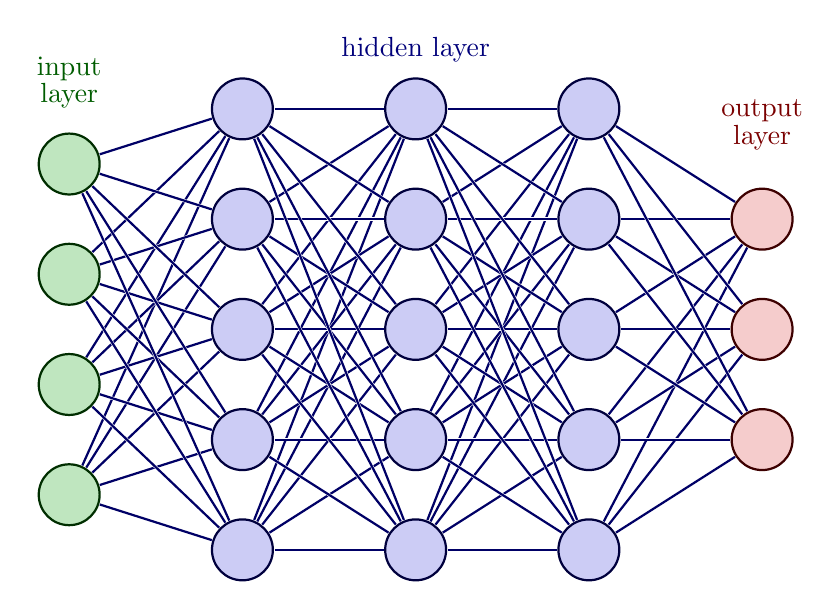
\begin{tikzpicture}[x=2.2cm,y=1.4cm]
      \message{^^JNeural network without text}
      \readlist\Nnod{4,5,5,5,3} % array of number of nodes per layer
      
      \message{^^J  Layer}
      \foreachitem \N \in \Nnod{ % loop over layers
        \def\lay{\Ncnt} % alias of index of current layer
        \pgfmathsetmacro\prev{int(\Ncnt-1)} % number of previous layer
        \message{\lay,}
        \foreach \i [evaluate={\y=\N/2-\i; \x=\lay; \n=\nstyle;}] in {1,...,\N}{ % loop over nodes
          
          % NODES
          \node[node \n] (N\lay-\i) at (\x,\y) {};
          
          % CONNECTIONS
          \ifnum\lay>1 % connect to previous layer
            \foreach \j in {1,...,\Nnod[\prev]}{ % loop over nodes in previous layer
              \draw[connect,white,line width=1.2] (N\prev-\j) -- (N\lay-\i);
              \draw[connect] (N\prev-\j) -- (N\lay-\i);
              %\draw[connect] (N\prev-\j.0) -- (N\lay-\i.180); % connect to left
            }
          \fi % else: nothing to connect first layer
          
        }
      }
      
      % LABELS
      \node[above=5,align=center,mygreen!60!black] at (N1-1.90) {input\\[-0.2em]layer};
      \node[above=2,align=center,myblue!60!black] at (N3-1.90) {hidden layer};
      \node[above=10,align=center,myred!60!black] at (N\Nnodlen-1.90) {output\\[-0.2em]layer};
      
    \end{tikzpicture}

    \end{center}
    \end{frame}


    \begin{frame}{Experiment}
      \begin{flushleft}
        MNIST dataset
      \end{flushleft}
      \begin{center}
          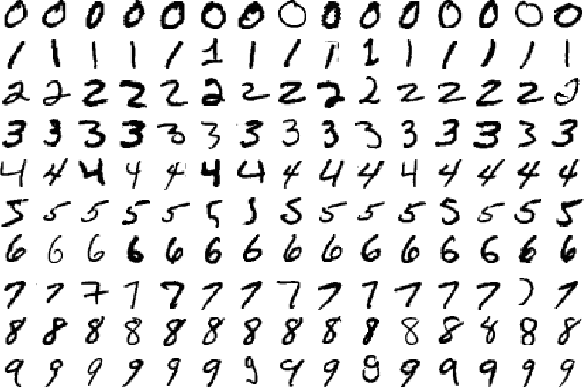
\includegraphics[scale=0.4]{/home/suzy/gitrepos/tuttelikz/221105/images/mnist.png}
      \end{center}
    \end{frame}
    
    \begin{frame}{Experiment}
      \centering
        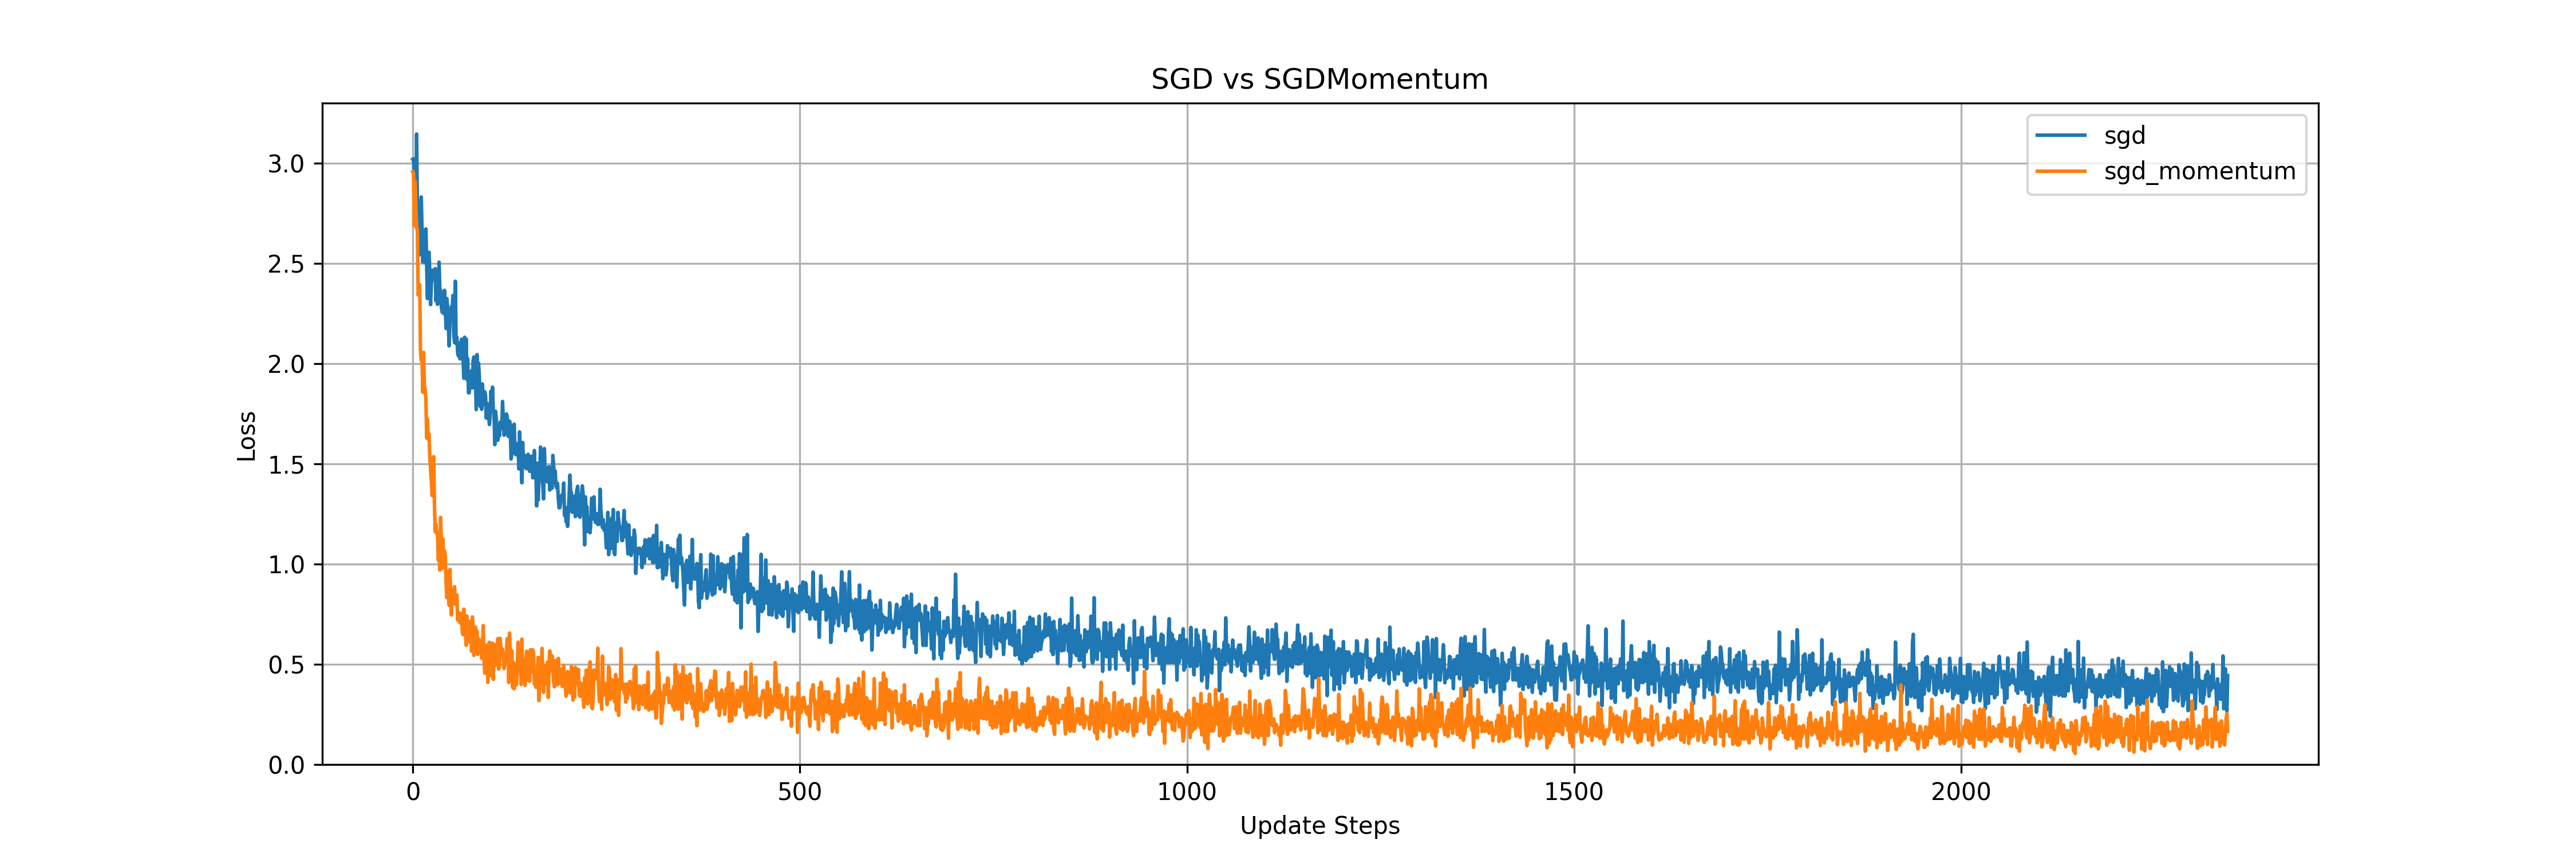
\includegraphics[width=1.0\textwidth]{/home/suzy/gitrepos/tuttelikz/221105/images/sgd_mom.png}
    \end{frame}

    % \begin{frame}[allowframebreaks]
    %   \frametitle{References}
    %   \bibliographystyle{amsalpha}
    %   \bibliography{/home/suzy/gitrepos/tuttelikz/221105/bibfile.bib}
    % \end{frame}
  \begin{frame}
    \printbibliography
  \end{frame} 
\end{document}


% @article{test1,
% title = {Commercial Banks as Creators of 'Money'},
% author = {Tobin, James},
% year = {1963},
% institution = {Cowles Foundation for Research in Economics, Yale University},
% number = {159},
% url = {http://EconPapers.repec.org/RePEc:cwl:cwldpp:159}
% }